\documentclass{article}
\usepackage[utf8]{inputenc}

\title{Algorithms Part 1}
\author{Farhan Sadeek}
\date{December 2022}
\usepackage{minted}
\usepackage{tikz}
\usepackage{listings}
\usepackage{xcolor} % to access the named colour LightGray
\definecolor{LightGray}{gray}{0.9}

\begin{document}
\maketitle

\section{Introduction}
In this course, we are going to learn about the most important algorithms for interviews in the world's largest tech-companies, such as Google, Apple, and Facebook. This course will teach you everything you need to know in order to excel in the data structures and algorithms course.

\section{Week 1}
\subsection{Quick Find}
Quick Find is an algorithm where we find if two nodes are connected to each other using the list of connected components.
\newline
\newline
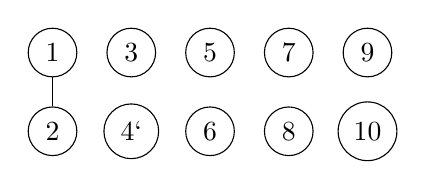
\begin{tikzpicture}[main/.style = {draw, circle}] 
\node[main] (1) {$1$}; 
\node[main] (2)[below of = 1]{$2$};
\node[main] (3)[right of = 1]{$3$};
\node[main] (4)[below of = 3]{$4`$};
\node[main] (5)[right of = 3] {$5$};
\node[main] (6)[below of = 5]{$6$};
\node[main] (7)[right of = 5]{$7$};
\node[main] (8)[below of = 7] {$8$};
\node[main] (9)[right of = 7]{$9$};
\node[main] (10) [below of = 9]{$10$};

\draw (1) -- (2);
\end{tikzpicture} 
Here is the code example java and C++.

\begin{minted}{java}
import java.util.*;
public class Quick_Find {
    private int id[];
    // set id of each object itself (N array access)
    public Quick_Find(int n){
        id = new int[n];
        for(int i = 0; i < n; i++){
            id[i] = i;
        }
    }
    // Check whether p and q have the same components
    public boolean connected(int p, int q){
        return id[p] == id[q];
    }

    public void union(int p, int q){
        int pid = id[p];
        int qid = id[q];
        for(int i = 0; i < id.length; i++){
            if(id[i] == pid){
                id[i] = qid;
            }
        }
    }
}
\end{minted}

Here in this code segment there are three portions: the constructor, the accessor and the mutator method.

\subsubsection{Constructor}
\begin{minted}{java}
public Quick_Find(int n){
    id = new int[n];
    for(int i = 0; i < n; i++){
        id[i] = i;
    }
}   
\end{minted}
The constructor method sets the value of all the address to it's original value considering the fact that every single node is connected to itself.

\subsubsection{Accessor}
\begin{minted}{cpp}
    public static boolean connected(int p, int q){
        return id[p] == id[q]; 
    }
\end{minted}
    
\subsection{Quick Union}
Quick Union is an algorithm where we find if two nodes are connected to each other using the list of nodes in a list.
\end{document}
